%\usepackage{extsizes}
\documentclass[14pt, a4paper, russian]{report}

\linespread{1.3}

\usepackage{titlesec}
\usepackage[centertags]{amsmath}
\usepackage{amsthm,amsfonts,amssymb}
\usepackage{indentfirst}

\usepackage{extsizes}
\usepackage[left=25mm,right=10mm,top=20mm,bottom=20mm,bindingoffset=0cm]{geometry}

\usepackage{cmap}
\usepackage{multirow}
\usepackage{float}
\usepackage{mathtools}
\DeclarePairedDelimiter\ceil{\lceil}{\rceil}
\DeclarePairedDelimiter\floor{\lfloor}{\rfloor}

\usepackage{qtree}

\usepackage[T2A]{fontenc}
\usepackage[utf8]{inputenc}
\usepackage[english,russian]{babel}
%\usepackage{pscyr}
\RequirePackage{graphicx}
\RequirePackage{subfig}
\RequirePackage{pgfplots}
\usepackage{thmtools}   
\usepackage{hyperref}
\usepackage[nameinlink]{cleveref}


\newtheorem{lemma}{\indent Лемма}
\newtheorem{theorem}{\indent Теорема}
\newtheorem{corollary}{\indent Следствие}
\newtheorem{problem}{\indent Задача}
\newtheorem{remark}{\indent Замечание}
\newtheorem{definition}{\indent Определение}
\newtheorem{proposition}{\indent Утверждение}
\newtheorem{example}{\indent Пример}
\newtheorem{notation}{\indent Обозначение}

\crefname{lemma}{л.}{л.}
\crefname{theorem}{теор.}{теор.}
\crefname{corollary}{след.}{след.}
\crefname{definition}{опр.}{опр.}
\crefname{proposition}{утв.}{утв.}
\crefname{example}{прим.}{прим.}
\crefname{notation}{обозн.}{обозн.}
\crefname{remark}{замеч.}{замеч.}

\crefname{theorem}{Теорема}{Теорема}
\newcommand{\order}[2]{#1_{(#2)}}

\newcommand{\T}{^{\text{\tiny\sffamily\upshape\mdseries T}}}

\graphicspath{{./img/}}


\def\XYtext(#1,#2)#3{\rlap{\kern#1\lower-#2\hbox{#3}}}

% Переопределение вставки графики
\newcounter{PictureNo}

\hyphenpenalty 100
\tolerance 10000


\newenvironment{Proof}%
    {\par\noindent{\bf Доказательство.}}%
    {\hfill$\scriptstyle\blacksquare$}

\usepackage{bbm}
\bibliographystyle{unsrt}

\addto\captionsenglish{\renewcommand{\figurename}{Рисунок}}
\addto\captionsenglish{\renewcommand{\tablename}{Таблица}}
\addto\captionsenglish{\renewcommand{\bibname}{Список использованных источников}}
\captionsetup[figure]{labelfont=footnotesize,textfont=footnotesize}
\captionsetup[table]{labelfont=footnotesize,textfont=footnotesize}

\addto\captionsenglish{\renewcommand{\proofname}{Доказательство}}

\makeatletter % эта строка НЕОБХОДИМА!
\renewcommand{\@chapapp}{Глава} 
\addto\captionsenglish{% Replace "english" with the language you use
  \renewcommand{\contentsname}%
    {Оглавление}%
}

\titleformat{\chapter}[display]
{\normalfont\bfseries\center}
{Глава \thechapter. }{0em}{}

\titleformat{\section}[block]
{\normalfont\bfseries\center}
{\thesection. }{0em}{}

\newcommand\thefontsize[1]{{#1 The current font size is: \f@size pt\par}}

\begin{document}
\begin{center}
\hfill \break
\small{Федеральное государственное автономное образовательное учреждение \linebreak 
высшего образования}\\ 
\small{<<Московский физико-технический институт (государственный университет)>>}\\
\hfill \break
\small{Факультет инноваций и высоких технологий}\\
\small{Кафедра анализа данных}\\
\end{center}
\small{\textbf{Направление подготовки:} 01.03.02 Прикладная математика и информатика}\\
\hfill \break
\hfill \break
\hfill \break
\hfill \break
\begin{center}
\normalsize{\textbf{Автоматическая расстановка ударений в словах}}\\
\small{Бакалаврская работа}\\
\hfill \break
\hfill \break
\end{center}
 
\hfill \break
 
\begin{flushright}
\small{ 
\begin{tabular}{rl}
\textbf{Обучающийся:} & ФИО \\
 & \underline{\hspace{3cm}} \\\\
\textbf{Научный руководитель:} & должность\\
            & ФИО \\
 & \underline{\hspace{3cm}} \\\\
\end{tabular}
}
\end{flushright}

\hfill \break
\hfill \break
\hfill \break
\hfill \break
\begin{center} Москва 2018 \end{center}
\thispagestyle{empty} % выключаем отображение номера для этой страницы
 
% КОНЕЦ ТИТУЛЬНОГО ЛИСТА
 
\newpage
\begin{normalsize}
\chapter*{Аннотация}


Умные слова в 1500 знаков


\tableofcontents{}


\chapter*{Введение}
\addcontentsline{toc}{chapter}{Введение}
Ударение в словах – важнейший элемент устной, письменной и внутренней речи. В русском языке оно играет исключительно важную роль, так как благодаря ему мы можем различать слова. Одной из сложностей русского языка является его свободное ударение, которое не закреплено за каким-либо определенным слогом или морфемой слова. Любой слог может выделяться фонетически. К тому же ударение  может меняться с изменением грамматической формы слова. Как отмечает лингвист Н. А. Еськова, «слова с подвижным ударением в русском языке исчисляются сотнями. В процентном отношении это немного, но среди них много чрезвычайно употребительных, поэтому в речи они достаточно заметны».\cite{eskina} Например: фл\'{а}г — фл\'{а}га — фл\'{а}ги; но вр\'{а}г — враг\'{а} — враг\'{и} 

Есть языки, где ударение  всегда на одном и том же слоге — такое ударение называют фиксированным. Например, во французском ударение всегда на последнем слоге, в польском — на предпоследнем, в чешском — на первом. В русском языке аналогичные правила весьма размыты, поэтому если человек не знает, как правильно ставить ударение в слове, то по одному только его внешнему облику сделать правильный выбор бывает сложно.  Нет общих правил ударения и в заимствованных для русского языка словах . Иногда оно меняет свое место по сравнению с ударением в языке-источнике: ноутб\'{у}к, скелет\'{о}н, футб\'{о}л, хокк\'{е}й. А иногда сохраняет: буль\'{о}н, гардер\'{о}б, жалюз\'{и}.
Расстановка ударений, как часть задачи предсказания произношения, - важная составляющая  приложений, таких как: автоматическое распознавание речи, синтез речи, транслитерация. Кроме того – это необходимо всем, изучающим русский язык.


\newpage

\chapter{Литературный обзор}

Работы по предсказанию постановки ударений в словах велись в двух направлениях. На основе лингвистических правил \cite{church, williams} и на основе анализа данных, где модели строятся напрямую из текстов с обозначенными ударениями. 

В русском языке сохраняется множество индо-европейских шаблонов ударений. Чтобы узнать ударение морфологически сложного слова, состоящего из основы и окончания, необходимо узнать является ли основа ударной и на какой слог падает в ней ударение, либо ударным является окончание. \cite{halle}
\section{Предсказание ударения в слове на основе ражирования}
Авторы\cite{hall} рассмотрели проблему расстановки ударений, как задачу ранжирования. В своем исследовании  они опирались на более раннюю статью\cite{dou}. Из каждого слова выделяются гласные буквы и они предполагаются, как возможные варианты постановки ударений. Целью модели является отранжировать варианты так, чтобы верная гипотеза имела наименьший ранг.

Для ранжирования гипотез применялось Maximum Entropy ранжирование.\cite{collins} Во время обучения модели ей подавался набор правильных гипотез и их признаков. Во время предсказания в модель подавались все гипотезы, и в качестве верной выбиралась гипотеза с максимальным предсказанным результатом. В качестве основы для ранжирования использовалась линейная модель, вместо SVM, так как она более эффективна с вычислительной точки зрения для обучения и применения. 

В базовой статье\cite{dou} признаками являлись триграммы для гласных букв следующего вида: предыдущая согласная, если она есть, гласная буква, следующая за ней слогласная, если она есть(Dou). На основе лигвистического исследования в данной статье авторы добавили следующие признаки для каждого слова взяты все его начала и концы (уже - у, уж, уже, е, же).(Affix) Также эти признаки добавлены в следующем виде: все буквы заменены на их абстрактные фонетические классы (представлены в \cref{table:phon_class})({Abstr Aff}).
\begin{table}[H]
	\begin{small}
		\begin{center}
			\begin{tabular}{|c|c|}
				\hline
				Класс & Буквы \\			
				\hline
				vowel & а, е, и, о , у, э, ю, я, ы \\
				\hline
				stop & б, д, г, п, т, к \\
				\hline
				nasal & м, н \\
				\hline
				fricative & ф, с, ш, щ, х, з, ж \\
\hline
				hard/soft & ъ, ь\\
\hline
				yo & ё \\
\hline
				semivowel & й, в \\
\hline
				liquid & р, л\\
\hline
				affricate & ц, ч \\
\hline
		
			\end{tabular}
		\end{center}
	\end{small}
	\caption{ Абстрактные фонетические классы.}
	\label{table:phon_class}
\end{table}

В качетсве данных авторы использовали Грамматический словарь русского языка\cite{zaliz}, разбитый на обучающую и тестовую выборки. Из тестовой выборки также были отдельно выделены те слова которые не встречались в обучающей выборке  и для них также были получены  результаты. Результаты экспериментов представлены в \cref{table:range_res}.
\begin{table}[H]
	\begin{small}
		\begin{center}
			\begin{tabular}{|c|c|}
				\hline
				Признаки & Accuracy score \\
				\hline
				\multicolumn{2}{|c|}{Тестовая выборка} \\			
				\hline
				Dou &0.972 \\
				\hline
				Aff & 0.987 \\
				\hline
				Aff+Abstr Aff & 0.987 \\
				\hline
				Dou et al+Aff & 0.987 \\
				\hline
				Dou et al+Aff+Abstr Aff & 0.987 \\
				\hline
				\multicolumn{2}{|c|}{Слова не встречавшиеся в обучающей выборке} \\			
				\hline
				Dou &0.806 \\
				\hline
				Aff & 0.798 \\
				\hline
				Aff+Abstr Aff & 0.810 \\
				\hline
				Dou et al+Aff & 0.823 \\
				\hline
				Dou et al+Aff+Abstr Aff & 0.89 \\
				\hline
				
			\end{tabular}
		\end{center}
	\end{small}
	\caption{Результаты ранжирования.}
	\label{table:range_res}
\end{table}

Таблица показывает  влияние взаимодействия признаков на обобщающую способность модели и лучший результат достигнут при использовании всех признаков.

Недостатками этой статьи является не использование контекста для определения места ударения, при подсчете результатов никак не учитывалась частота употребления слов в текстах языка, использовался просто его лексический набор.

\section{Предсказание ударения в слове при помощи помощи конечного преобразователя}

Целью авторов\cite{reynolds} было разработки модели, которая могла быть помочь людям изучать русский язык, они решили что в некоторых словах ударение может быть пропущено, так как неправильное ударение может быть хуже, чем его отсутствие для человека.

Модель состояла из двух частей: конечного преобразователя\cite{koskenniemi, karttunen}, который из полученного слова генерировал все возможные, корректные по его мнению позиции ударения. Далее при помощи формальной грамматики\cite{karlsson} удалялись варианты которые не подходили по контексту. Если после применения этой процедуры оставался один вариант прочтения, то он и выбирался как финальный, если ни одного, то ударение в слове не проставлялось, если же их было несколько, то в зависимости от эксперимента выбиралась дальнейшая стратегия. 

Авторами использовался корпус текстов состоящий из 7689 слов с размеченными ударениями, это тексты для начинающих изучать русский язык. Также для обучения модели применялся Грамматический словарь русского языка Зализняка\cite{zaliz}. 

Описание экспериментов:
\begin{itemize}
	\item \textbf{bare:} при нескольких возможных прочтениях  слова, ударение в слове не проставлялось.
	\item \textbf{safe:}  при нескольких возможных прочтениях, ударение в слове выставлялось, если в них всех ударение падало на один и тот же слог.
	\item \textbf{randReading:} при нескольких возможных прочтениях, случайно выбиралось одно с вероятностью выбора варианта равной частоте встречаемости этого варианта в тексте.
	
	\item \textbf{freqReading:} при нескольких возможных прочтениях, выбирается вариант с максимальной  частотой встречаемости среди всех  вариантов в тексте.
\end{itemize}


Эксперименты были проведены при использовании формальной грамматики для учитывания контекста и без него. Результаты представлены в \cref{table:final_state_result}. Для слов,которые не встретились в словаре, применялось простое правило постановки ударения: ударение падает на последню гласную, после которой идет согласная. Это является наиболее вероятным вариантом ударения в русском языке\cite{lavitskaya}. В результатх это отображено как guessSyl.

\begin{table}[H]
	\begin{small}
		\begin{center}
			\begin{tabular}{|c|c|c|c|}
				\hline
				Экспериимент & Accuracy score & Доля Ошибок & Доля пропущенных слов\\
				\hline
				\multicolumn{4}{|c|}{Без грамматики} \\			
				\hline
				bare & 30.43 & 0.17 & 69.39 \\
				\hline
				safe & 90.07 & 0.49 & 9.44 \\
				\hline
				randReading &94.34 &3.36 &2.30 \\
				\hline
				freqReading &95.53 &2.59& 1.88 \\
				\hline
				randReading+guessSyll &94.99 &4.05 &0.96 \\
				\hline
				freqReading+guessSyll & 95.83 &3.46 &0.72\\
				\hline
				\multicolumn{4}{|c|}{С грамматикой} \\			
				\hline
				bare &45.78 & 0.44 &53.78\\
				\hline
				safe &93.21& 0.74 &6.058 \\
				\hline
				randReading &95.50 &2.59 &1.90 \\
				\hline
				freqReading &95.73 &2.40 &1.88 \\
				\hline
				randReading+guessSyll &95.92 &3.33 &0.74 \\
				\hline
				freqReading+guessSyll &96.15 &3.14 &0.72 \\
				\hline
				
			\end{tabular}
		\end{center}
	\end{small}
	\caption{Результаты применения конечного преобразователя.}
	\label{table:final_state_result}
	
\end{table}

При использовании модели без формальной грамматики среди полнота гипотез составила 97.55\%, что является максимумом результата для данной модели. При использовании грамматики полнота составила 97.35\%. Эти результаты являются потолком для соответствующих экспериментов. Совмещение всех моделей и предсказываение методом FreqReading  позволило получить наибольших процент угаданных слов. Метод расстановки ударений для неизвестных слов в данном случае имеет точность всего 21\%. При этом высокая точность была достигнута за счет расстановки ударений почти во всех словах, что соответственно повысило уровень ошибок. 

Метод, представленный в этой статье, является попыткой улучшить словарный метод, путем разрешения неоднозначностей в омографах при помощи формальной грамматики. При этом для слов, которые не  встретились в словаре работает очень простой и слабый алгоритм, в этом случае качество получается очень низким. Недостатком является также использование небольшого закрытого корпуса текстов, при этом, так как это тексты для начинающих, их словарь скорее всего был достаточно мал. Также проведение экспериментов RandReading и FreqReading непонятно, так как несложно показать строго математически, что метод FreqReading всегда дает большую вероятность правильного ответа.

\section{Предсказание ударения в слове при помощи символьной нейронной сети}
	В качестве основы для модели авторы\cite{ponomareva} использовалась  символьная двусторонняя рекуррентная нейронная сеть на основе LSTM-модулей. На вход подавалась матрица размера [длина фразы; число возможных символов]. Для кодирования символов было применено one-hot кодирование. Авторами выбрана следующая архитектура: к входной матрице применяется двусторонняя рекуррентная нейронная сеть, сконкатенированные вектора, полученные от рекуррентного слоя подаются в полносвязные слой с softmax активацией. На выходе получается вектор размера длина фразы, соответствующий распределению вероятностей поставить ударение в конкретной позиции.(представлена на \cref{fig:base_global})

\begin{figure}[H]
	\begin{center}
		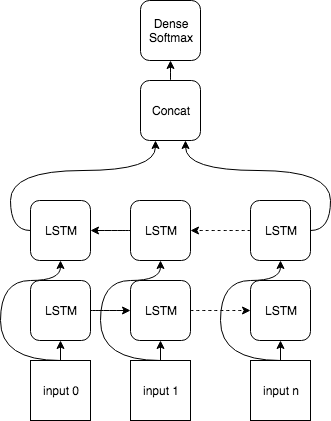
\includegraphics[width=0.5\linewidth]{Baseline}
	\end{center}
	\caption{\small{Архитектура сети}}
	\label{fig:base_global}
\end{figure}

Для разных экспериментов использовался грамматический словарь русского языка Зализняка,\cite{zaliz} и база данных акцентологической разметки в составе национального корпуса русского языка\cite{grishina} 

Авторами были проведены следующие эксперименты
\begin{enumerate}
	\item \textbf{Обучение и предсказание на основе словаря.} Словарь Зализняка был разделен на обучающую и тестовую выборки в соотношении 2:1. Результаты этого эксперимента представлены в \cref{table:dict_res}.
	\item \textbf{Обучение и предсказание на основе акцентологического корпуса.} С корпусом было проведено два эксперимента, в первом в качестве фразы использовалось только само слово. Во втором же, к нему были дописаны три последние буквы из слова, которое идет перед ним в предложении, если такое было. Сравнительные результаты экспериментов представлены в \cref{table:base_text}. Основная разница между моделями с контекстом и без него может быть видна только на омографах. Результаты применения на них представлены в \cref{table:base_homo}. Как видно из результатов модель успешно использует контекст для расстовки ударения в омографах во многих случаях.
\end{enumerate}

\begin{table}[H]
	\begin{small}
		\begin{center}
			\begin{tabular}{|c|c|c|c|}
				\hline
				Экспериимент & Accuracy score & Доля Ошибок & Доля пропущенных слов\\
				\hline
				\multicolumn{4}{|c|}{Без грамматики} \\			
				\hline
				bare & 30.43 & 0.17 & 69.39 \\
				\hline
				safe & 90.07 & 0.49 & 9.44 \\
				\hline
				randReading &94.34 &3.36 &2.30 \\
				\hline
				freqReading &95.53 &2.59& 1.88 \\
				\hline
				randReading+guessSyll &94.99 &4.05 &0.96 \\
				\hline
				freqReading+guessSyll & 95.83 &3.46 &0.72\\
				\hline
				\multicolumn{4}{|c|}{С грамматикой} \\			
				\hline
				bare &45.78 & 0.44 &53.78\\
				\hline
				safe &93.21& 0.74 &6.058 \\
				\hline
				randReading &95.50 &2.59 &1.90 \\
				\hline
				freqReading &95.73 &2.40 &1.88 \\
				\hline
				randReading+guessSyll &95.92 &3.33 &0.74 \\
				\hline
				freqReading+guessSyll &96.15 &3.14 &0.72 \\
				\hline
				
			\end{tabular}
		\end{center}
	\end{small}
	\caption{Результаты применения нейросетевой моделе на словаре Зализняка.}
	\label{table:dict_res}
\end{table}

\begin{table}[H]
	\begin{small}
		\begin{center}
			\begin{tabular}{|c|c|c|c|}
				\hline
				Экспериимент & Accuracy score & Доля Ошибок & Доля пропущенных слов\\
				\hline
				\multicolumn{4}{|c|}{Без грамматики} \\			
				\hline
				bare & 30.43 & 0.17 & 69.39 \\
				\hline
				safe & 90.07 & 0.49 & 9.44 \\
				\hline
				randReading &94.34 &3.36 &2.30 \\
				\hline
				freqReading &95.53 &2.59& 1.88 \\
				\hline
				randReading+guessSyll &94.99 &4.05 &0.96 \\
				\hline
				freqReading+guessSyll & 95.83 &3.46 &0.72\\
				\hline
				\multicolumn{4}{|c|}{С грамматикой} \\			
				\hline
				bare &45.78 & 0.44 &53.78\\
				\hline
				safe &93.21& 0.74 &6.058 \\
				\hline
				randReading &95.50 &2.59 &1.90 \\
				\hline
				freqReading &95.73 &2.40 &1.88 \\
				\hline
				randReading+guessSyll &95.92 &3.33 &0.74 \\
				\hline
				freqReading+guessSyll &96.15 &3.14 &0.72 \\
				\hline
				
			\end{tabular}
		\end{center}
	\end{small}
	\caption{Результаты применения нейросетевой моделе на словаре Зализняка.}
	\label{table:base_text}
\end{table}

\begin{table}[H]
	\begin{small}
		\begin{center}
			\begin{tabular}{|c|c|c|c|}
				\hline
				Экспериимент & Accuracy score & Доля Ошибок & Доля пропущенных слов\\
				\hline
				\multicolumn{4}{|c|}{Без грамматики} \\			
				\hline
				bare & 30.43 & 0.17 & 69.39 \\
				\hline
				safe & 90.07 & 0.49 & 9.44 \\
				\hline
				randReading &94.34 &3.36 &2.30 \\
				\hline
				freqReading &95.53 &2.59& 1.88 \\
				\hline
				randReading+guessSyll &94.99 &4.05 &0.96 \\
				\hline
				freqReading+guessSyll & 95.83 &3.46 &0.72\\
				\hline
				\multicolumn{4}{|c|}{С грамматикой} \\			
				\hline
				bare &45.78 & 0.44 &53.78\\
				\hline
				safe &93.21& 0.74 &6.058 \\
				\hline
				randReading &95.50 &2.59 &1.90 \\
				\hline
				freqReading &95.73 &2.40 &1.88 \\
				\hline
				randReading+guessSyll &95.92 &3.33 &0.74 \\
				\hline
				freqReading+guessSyll &96.15 &3.14 &0.72 \\
				\hline
				
			\end{tabular}
		\end{center}
	\end{small}
	\caption{Результаты применения нейросетевой моделе на омографах.}
	\label{table:base_homo}
\end{table}

Как видно нейросетевая модель успешно справляется с использование контекста для расстановки ударений в омографах. Недостатками же представленной модели является очень простая архитектура и отсутствие работы с текстом. Далее мы будем использовать эту модель как базовую для сравнения результатов. 


\newpage
\chapter{Tmp}
\section{Основные обозначения и определения}

Все говорят: Кремль, Кремль. Ото всех я слышал про него, а сам ни разу не видел. Сколько раз уже (тысячу раз), напившись или с похмелюги, проходил по Москве с севера на юг, с запада на восток, из конца в конец, насквозь и как попало – и ни разу не видел Кремля \cite{erofeev}.

\begin{definition}\label{def:schizo}
Шизофазия (речевая разорванность) - симптом психических расстройств, выражающийся в нарушении структуры речи, при которой, в отличие от речевой бессвязности (потока несвязанных слов), фразы строятся правильно, однако не несут никакой смысловой нагрузки, а содержание речи соответствует содержанию бреда.\cite{schizo}
\end{definition}
$$E = m c^2$$

\begin{notation} 
\begin{itemize}
\item $H$ --- водород.
\item $O$ --- кислород.
\item $C$ --- углерод.
\item $\ldots$
\end{itemize}
\end{notation}

На формулки тоже можно ссылаться.

\begin{equation}\label{eq:women}
Women = Evil
\end{equation}

Согласно (\ref{eq:women}), женщины --- зло.

Собсно, на все леммы, теоремы, примеры, замечания и тэдэ можно ссылаться.

\begin{example}\label{ex:ivanova}
Вот, например, Лёшка хотел Отл(10), а Иванова ему 9 поставила.
\end{example}

\begin{remark}\label{rem:gertsen}
Родился на улице Герцена, в гастрономе номер двадцать два. Известный экономист, по призванию своему — библиотекарь. В народе — колхозник. В магазине — продавец. В экономике, так сказать, необходим. Это, так сказать, система… э-э-э… в составе ста двадцати единиц. Фотографируете Мурманский полуостров и получаете «Те-ле-фун-кен». И бухгалтер работает по другой линии — по линии библиотекаря. Потому что не воздух будет, академик будет! Ну вот можно сфотографировать Мурманский полуостров. Можно стать воздушным асом. Можно стать воздушной планетой. И будешь уверен, что эту планету примут по учебнику. Значит, на пользу физике пойдёт одна планета. \cite{schizo}
\end{remark}

В силу \cref{ex:ivanova} и \cref{rem:gertsen}, динозавры вымерли.


\section{Ещё какая-то муть}
Так. Стакан зубровки. А потом – на Каляевской – другой стакан, только уже не зубровки, а кориандровой. Один мой знакомый говорил, что кориандровая действует на человека антигуманно, то есть, укрепляя все члены, ослабляет душу. Со мной почему-то случилось наоборот, то есть душа в высшей степени окрепла, а члены ослабели, но я согласен, что и это антигуманно. Поэтому там же, на Каляевской, я добавил еще две кружки жигулевского пива и из горлышка альб-де-дессерт.\cite{erofeev}



\chapter{Заметки о женской логике}
\section{Как говорил Бек}
В наш век точное познание завоевывает все новые области. Одна из таких областей – женская логика. Строгое изложение находится еще в стадии зарождения. Обычная мужская логика прошла эту стадию более двух тысяч лет назад, но женская логика еще ждет своего Аристотеля. Потомкам принадлежит большая и почетная задача создать систематический курс женской логики, выполнить ее аксиоматизацию, создать вычислительные машины, действующие по женским логическим схемам.\cite{bek}

\begin{figure}[H]
	\begin{center}
		 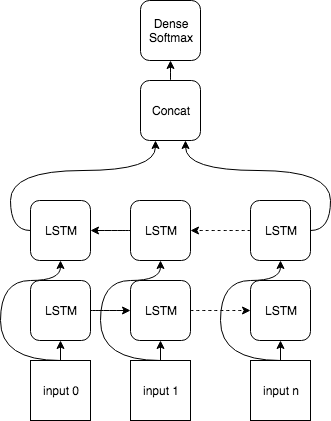
\includegraphics[width=0.5\linewidth]{Baseline}
	\end{center}
  
    \caption{\footnotesize{Чёрный квадрат}}
\label{fig:square}
\end{figure}

На картинку тоже можно ссылаться: \cref{fig:square}

\section{Теорема Сосницкого}
Следующая теорема даёт ответы на все ваши вопросы.

\begin{theorem}[Теорема Сосницкого]\label{th:sosnitsky}
Lorem ipsum dolor sit amet, consectetur adipiscing elit.
\end{theorem}

Для доказательства теоремы понадобится следующая лемма:

\begin{lemma}\label{le:sosnyakovsky}
Если в кране нет воды, значит выпили жиды.
\end{lemma}
\begin{proof}
Если в кране есть вода, значит жид нассал туда.

\end{proof}

\begin{enumerate}
\item Пер.
\item Пер.
\item Пер.
\end{enumerate}

\begin{corollary}\label{cor:erofeev}
О, тщета! О, эфемерность! 
\end{corollary}
\begin{proof}
О, самое бессильное и позорное время в жизни моего народа – время от рассвета до открытия магазинов! Сколько лишних седин оно вплело во всех нас, в бездомных и тоскующих шатенов!
\end{proof}

\chapter{Как рисовать всякие красивости}

\section{Система нумерованных уравнений}
\begin{align}
\label{eq:adin} \frac{dq}{dt} &= \frac{dH}{dp} \\
\label{eq:dva} \frac{dp}{dt} &= -\frac{dH}{dq}
\end{align}
А всё для того, чтобы сослаться раз (\ref{eq:adin}), сослаться два (\ref{eq:dva})
\begin{table}[H]\label{table:rokk_ebol}
\begin{small}
\begin{center}
\begin{tabular}{|c|c|c|c|}
\hline
Р & О & К & К\\
\hline
Е & Б & О & Л\\
\hline
М & У & П & Ю\\
\hline
О & В & И & Ч\\
\hline
Н & И & R & Е\\
\hline
Т &   &   & Й\\
абсв & & & \\
\hline
\end{tabular}
\end{center}
\end{small}
\caption{ Sample text.}

\end{table}

Что бы вы думали можно сделать с \cref{table:rokk_ebol}

\section{Дерево}
Хер знает зачем, но вдруг пригодится.

\begin{figure}[H]
\Tree[.(start) [.РОКК  [.р [.о [.к ] ] ]
                        [.к [.е [.б ] ]
                                [.о [.л ] ] ] ]
               [.ЕБОЛ  [.Lorem [.Ipsum [.Dolor ] ] ]
                        [.Set [.Amet [.fgs ] ]
                                [.fds [.foobar ] ] ] ]
               [.МУПЮ ]
               [.ОВИЧ [.раз [.раз [.раз ] ] ]
                           [.это [.хард [.басс ] ]
                                       [.саня [.колбасёр ] ] ] ] ]
    \caption{\footnotesize{Смотри как умею}}
\label{fig:tree}
\end{figure}
Опа \cref{fig:tree}. 

\chapter*{Заключение}
Несмотря на то, что можно это объяснить по-разному, хотя и в растерянности относительно возможных непониманий того, что следует из того, почему современные госпитали, и притом многие, с определенным и, вместе с тем неопределенным недоверием не выразили почти никакой заинтересованности в таком деле, как местная анестезия, и с полной уверенностью я при данных обстоятельствах не думаю, что стоит пытаться защищать не защищаемую репутацию хирургии вместо того, чтобы постараться привлечь на свою сторону других всяких разных, и это побудило меня несколько месяцев тому назад написать на эту тему большую часть чего-то вроде частично исчерпывающей статьи, закончить которую мне помешало плохое здоровье...
\newpage
\bibliography{references}

\end{normalsize}

\end{document}
